% 电磁波的传播

\section{电磁波的传播}
电磁波的传播本质上是波动方程的边值问题。
由无源的 Maxwell 方程组
\begin{subequations}
\begin{align}
  \curl \vb{E} = - \pdv{\vb{B}}{t} \\
  \curl \vb{B} =  \mu_0 \epsilon_0 \pdv{\vb{E}}{t} \\
  \div \vb{\vb{E}} =0 \\
  \div \vb{\vb{B}} =0 
\end{align}
\end{subequations}
得到电磁场的波动方程:
\begin{equation}
  \left\{
  \begin{aligned}
  &\Da{\vb{E}} =0 \\
  &\Da{\vb{B}} =0.
  \end{aligned}\right.
  \label{eq:电磁场的波动方程}
\end{equation}
将 Trail solution \(\vb{E}(\vb{r}, t) = \vb{E}(\vb{r}) e^{-i\omega t}\) 代入
\cref{eq:电磁场的波动方程},变为 Helmholtz equation:
\begin{equation}
  \left\{
  \begin{aligned}
  &\laplacian \vb{E} + k^2 \vb{E} =0 \\
  &\laplacian \vb{B} + k^2 \vb{B} =0.
  \end{aligned}\right.
  \label{eq:Helmholtz_equation}
\end{equation}
Helmholtz equation 事实上是\emph{时谐场}的波动方程。
具体推导见 \href{../drafts/Helmholtz_equation.xopp}{Helmholtz equation.xopp}。

在\(t\)时刻,在\(x\)的位置,有某个波阵面的相位为\(\phi\)。
在\(t\)时刻,
相位为\(\phi\)的波阵面,在\(x\)的位置。
经过\(\Delta t\)的时间间隔,
在\(t+\Delta t\)时刻,
相位为\(\phi\)的波阵面,从\(x\)的位置,移动到了\(x+\Delta x\)的位置。
相位为\(\phi\)的波阵面,移动的速度为\(\Delta x /  \Delta t\)。
\begin{equation}
  k x - \omega t = \text{constant}
\end{equation}
两边同时微分
\begin{equation}
  k \dd{x} - \omega \dd{t} = 0
\end{equation}
所以相速度(波阵面的移动速度)
\begin{equation}
v_p = \dv{x}{t} = \frac{\omega}{k}
\end{equation}
波数 \(k=\omega / v = 2 \pi / \lambda\) 为一个\(2 \pi\)相位内包含的波长个数。
波长\(\lambda\)为一个完整波形的长度。
由波动方程表达式知
\begin{equation}
v_p=
\frac{1}{\sqrt{\mu \epsilon}}
=
\frac{c}{\sqrt{\mu_r \epsilon_r}}
=\frac{c}{n}
\end{equation}
\begin{definition}[折射率]
\begin{equation}
  n = \sqrt{\mu_r \epsilon_r} 
\end{equation}
方向沿\(\vb{k}\)方向
\end{definition}

\begin{center}
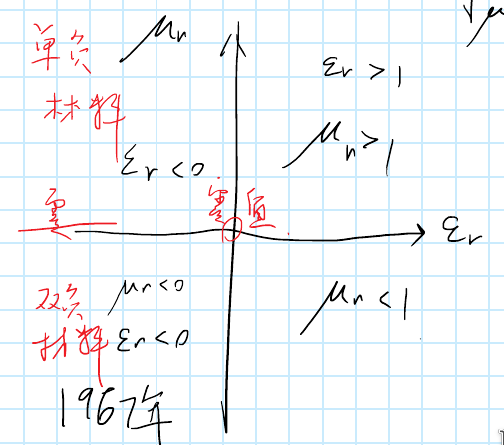
\includegraphics[width=0.5\textwidth]{figures/2022-11-14T221055+0800.png}
\captionof{figure}{实验上}
\end{center}

\(\omega_{pe}\) 等离子体振荡频率
\(\Omega_i\) 离子回旋频率
\(\Omega_e\) 电子回旋频率
\(\omega_{pe} > \Omega_i \)
\sn{频率再高一点的波,磁流体方程就不行了。}





%%% vim: set ts=2 sts=2 sw=2 isk+=\: et cc=+1 formatoptions+=mM:
